\chapter{Introdução}

\label{CapIntro}

Durante o desenvolvimento do trabalho de graduação ``Instrumentação e Controle de Braço Robótico para Deficientes'' foi
proposto um modelo com um determinado conjunto de parâmetros Denavit-Hartenberg. Este adendo buscará sanar dúvidas 
restantes quanto ao modelo desenvolvido e a convenção adotada para o posicionamento dos sistemas de coordenadas no 
manipulador.

A figura \ref{fig:DH-Novo} ilustra o modelo, com todos os parâmetros.

\begin{figure}[htb]
    \caption{Novo arranjo de sistemas.}    
    \begin{centering}

        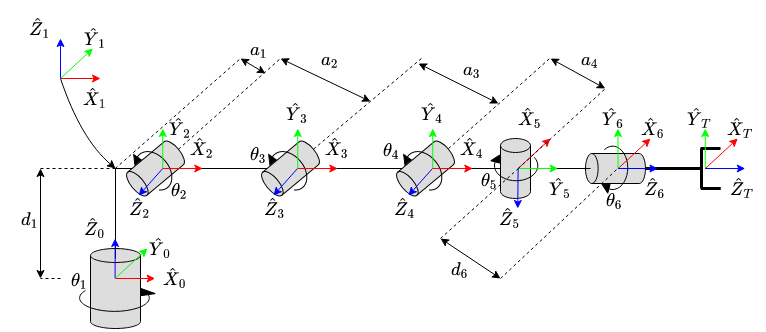
\includegraphics[width=1\columnwidth]{../images/arm/RefFrames.png}
    
    \par\end{centering}

    \label{fig:DH-Novo}
\end{figure}